\subsection{Tropical linear algebra}

%
%Fino a qui niente a capo
%
%Fino a qui niente a capo
%
%Fino a qui niente a capo
%
%Fino a qui niente a capo
%
%Fino a qui niente a capo
%
%Limite! Alla prossima riga sforo oltre 12 pag.
%

%In the next section we recall some basic ideas from tropical mathematics, and its connection with the study of the Lawvere quantale.
%Since polynomials correspond to piecewise linear (hence Lipschitz) functions in tropical mathematics,
%The reconstruction of the relational semantics over the tropical semi-ring, presented in Section \ref{section3} and Section \ref{section4}, will provide a metric semantics of the differential $\lambda$-calculus, bridging sensitivity and resource analysis. 
%In Section \ref{section5} we suggest potential applications of this approach, relating well-studied applications of program metrics, resource analysis with current uses of tropical mathematics in computer science.  
%Finally, in Section \ref{section6} we show that the connection between the metric and differential analysis of higher-order programs extends well beyond the relational semantics, through a more abstract correspondence between {generalized metric spaces} and modules over the tropical semiring.


%At the basis of our approach is the observation that the \emph{tropical semiring} $([0,\infty], \min, +)$, which is at the heart of tropical mathematics, coincides with the \emph{Lawvere quantale} $\Lawv=([0,\infty], \geq, +)$ \cite{Hofmann2014, Stubbe2014}, the structure at the heart of the categorical study of metric spaces initiated by Lawvere himself \cite{Lawvere1973}.
%Let us recall that a quantale is a complete lattice endowed with a continuous monoid action. In the case of $\Lawv$ the lattice is defined by the reverse order $\geq$ on $\BB R$, and the monoid action is provided by addition. Notice that the lattice join operation of $\Lawv$ coincides with the idempotent semiring operation $\min$. 
%A consequence of these observations is that, as we discussed below, the tropical approach to linear algebra coincides with the study of ``$\Lawv$-valued matrices'', i.e.~of maps of the form $s: X\times Y\to \Lawv$ .
%In particular, a (possibly $\infty$) metric on a set $X$ is nothing but a ``$\Lawv$-valued square matrix'' $d:X\times X\to \Lawv$ satisfying axioms like e.g.~the triangular law (indeed, such distance matrices correspond to $\Lawv$-\emph{enriched categories}, a viewpoint we explicitly take in Section \ref{section6}). 

%The study of matrices with values over the tropical semiring can be seen as a special case of the \emph{quantitative relational semantics} \cite{Manzo2013}, a well-studied semantics of the $\lambda$-calculus. 

A \emph{continuous} semiring \cite[Def. II.5]{Manzo2013} is a cpo equipped with an order-compatible semiring structure.
In a continuous semiring, all series always converge as $\sup$ of its partial sums.
%This is crucial for the definition of the weighted relational models for the $\lambda$-calculus.

\begin{example}
$[0,\infty]$ is a continuous semiring, which we denote $\overline{R_{\geq 0}}$, with usual order and semiring structure.
Notice that $\infty$ is added to ``artificially'' force any infinite series to converge.
The continuous semiring that we will use throughout all this paper is (one of) the so-called \emph{tropical semiring} $\Lawv:=[0,\infty]$ with $\min$ as sum (notice that it is idempotent) and $+$ as product.
Not only $\Lawv$ is at the heart of tropical mathematics, but it also coincides with the \emph{Lawvere quantale} \cite{Hofmann2014, Stubbe2014}
%(remember that a quantale is a complete lattice, for $\Lawv$ the order is $\geq$, endowed with a continuous monoidal action, for $\Lawv$ it is $+$)
, the structure at the heart of the categorical study of metric spaces initiated by Lawvere himself \cite{Lawvere1973}. 
%Notice that the lattice join operation of $\Lawv$ coincides with the idempotent semiring operation $\min$. 
\end{example}

For $Q$ a continuous semiring, one lets the category $\QREL$ (\cite{Manzo2013} calls it $Q^\Pi$) have sets as objects and set-indexed matrices with coefficients in $Q$ as morphisms, i.e.~$\QREL(X,Y):=Q^{X\times Y}$.
%The identity morphism of $\QREL$ is the identity matrix $I\in Q^{X\times X}$,
% given by $i_{a,a}=1$ and $i_{a,b\neq a}=0$, and
The composition $st\in Q^{X\times Z}$ of $t\in Q^{X\times Y}$ and $s\in Q^{Y\times Z}$ is given by $(st)_{a,c}:=\sum_{b\in Y} s_{b,c}t_{a,b}$ (such series converges because $Q$ is continuous).
As expected, $Q^X$ is a $Q$-semimodule and we identify $\HOM{\QREL}{X}{Y}$ with the set of linear maps from $Q^X$ to $Q^Y$, which have shape $f(x)_b=:\sum_{a\in X} \matr f_{a,b}x_a$, for some matrix $\matr f\in Q^{X\times Y}$.
% \begin{remark}
 %Following \cite{Manzo2013, Hofmann2014, Ehrhard2005}, we chose to see a matrix $t$ from $X$ to $Y$ as a map $t:X\times Y\to Q$.
% 
% fix $\HOM{\QREL}{X}{Y}:=Q^{X\times Y}$ with composition $st:X\times Z\to Q$ of $s:Y\times Z\to Q$ and $t:X\times Y\to Q$ defined by $(st)_{a,c}:=\sum_{b\in Y} s_{b,c}t_{a,b}$.
Notice that usual linear algebra conventions correspond to work in $\QREL^{\op}$, %a matrix $X\times Y\to Q$ is usually called a ``$Y\times X$-matrix'', meaning $Y$ rows and $X$ columns
e.g.\ the usual matrix-vector product defines a map $Q^Y\to Q^X$.
Following \cite{Manzo2013, Hofmann2014, Ehrhard2005}, we are instead working with transpose matrices.
%\end{remark}
%
%In $\QREL^{op}$ (which corresponds to systematically taking transpose matrices), composition coincides with the product matrix/matrix and $\hat{(\cdot)}$ with the product matrix/vector.
%In order to avoid confusion, we will refer to a $t\in Q^{X\times Y}$ just as a \emph{matrix from $X$ to $Y$}.
%
%
%
%We must fix a convention for matrices: following \cite{Manzo2013, Hofmann2014, Ehrhard2005}, we fix $\HOM{\QREL}{X}{Y}:=Q^{X\times Y}$ with composition $st:X\times Z\to Q$ of $s:Y\times Z\to Q$ and $t:X\times Y\to Q$ defined by $(st)_{a,c}:=\sum_{b\in Y} s_{b,c}t_{a,b}$.
%In linear algebra, a map $X\times Y\to Q$ is usually called a ``$Y\times X$-matrix'', meaning $Y$ rows and $X$ columns.
%In particular, the product of such a matrix for a vector defines a map $Q^Y\to Q^X$.
%Instead, we prefer to see a $t\in\HOM{\QREL}{X}{Y}$ as giving rise to a map $\hat t:Q^X\to Q^Y$ defined by $\hat t(x)_a:=\sum_{b\in Y} t_{a,b}x_a$.
%In $\QREL^{op}$ (which corresponds to systematically taking transpose matrices), composition coincides with the product matrix/matrix and $\hat{(\cdot)}$ with the product matrix/vector.
%In order to avoid confusion, we will refer to a $t\in Q^{X\times Y}$ just as a \emph{matrix from $X$ to $Y$}.
%As it is expected, $Q^X$ is a $Q$-semimodule and the bijection $\hat{(\cdot)}$ identifies $\HOM{\QREL}{X}{Y}$ with the set of linear maps from $Q^X$ to $Q^Y$.

The main actor of this paper is the category $\LREL$. % of sets and matrices with values over $\Lawv$ (which is a continuous semi-ring).
%, where $\Lawv$ is the already introduced Lawvere quantale, seen as the idempotent complete semiring $(\BB R_{\geq0}\cup\set{\infty},\inf,\infty,+,0)$.
%The category $\LREL$ is well-defined because $\Lawv$ is a continuous semiring (w.r.t.\ its quantale order $\preceq$.
%This amounts to check that $\min$ and $+$ commute with the $\inf$ (as operations on $\BB R_{\geq0}\cup\set{\infty}$, which is immediate), and that $(\Lawv,\preceq)$ is a cpo with $\infty$ as bottom element (which is immediate since in $\Lawv$ we have $\vee = \inf$) .
It is worth observing that the composition in $\LREL$ %is the tropicalisation of the one defining it in $\QREL$, i.e.
reads as \ $(st)_{a,c}:=\inf_{b\in Y}\set{s_{b,c}+t_{a,b}}$;
similarly, the linear functions $f:\Lawv^X\to \Lawv^Y$, %induced by matrices
which we call \emph{tropical linear}, are exactly those of shape $f(x)_b=\inf_{a\in X} \set{\matr f_{a,b}+x_a}$, for some $\matr f\in\Lawv^{X\times Y}$.
%\end{remark}

%Since $\Lawv$ is a continuous commutative semiring, [Proposition III.3, \cite{Manzo2013}] immediately applies and gives:

%\begin{proposition}
% $\LREL$ is a linear $\Lawv$-category.
%\end{proposition}

%Unwrapping [Definition II.9, \cite{Manzo2013}], this means that:
%$\HOM{\LREL}{X}{Y}$ is a continuous $\Lawv$-semimodule, with semimodule operations defined pointwise;
%$\LREL$ is a continuous $\Lawv$-category, i.e.\ composition of morphisms commutes with $\inf$'s;
%$\LREL$ is linear, i.e.\ pre- and post-composition with any morphism in any $\HOM{\LREL}{X}{Y}$ are automorphisms on it.

%In the next sections we will see how $\LREL$ gives rise to denotational models of several variants of the $\lam$-calculus.



%
%
%
% 

%
%
%or more generally as a power series $f(x)=\sum_{n}\widehat f_{n}x^{n}$ with coefficient $\widehat f_{n}\in [0,1]$, we can define its \emph{tropicalization} $\trop f: \Lawv \to \Lawv$ as the function 
%\begin{align}
%\trop f(\alpha)= \inf_{n}\left\{ 
%\end{align}
%
%This correspondence can be made precise through the the so-called
% \emph{de Maslov dequantization} \cite{}.
% For each positive real $t$, any polynomial in $\BB R[x]$ can be written under the \emph{$t$-parameterized} form:
% \begin{align}
% p_{t}(x)= \sum_{i=1}^{k}t^{c_{i}}x^{i}
% \end{align}
% with the coefficients $c_{i}$ taken from $\Lawv$. 
% It is clear then that tropical polynomials and $t$-parameterized polynomials admit a one to one correspondence between their presentations.
% 
% Actually, the $\varphi$s and the $p_{t}$s can be related by passing through some intermediate functions $\varphi_{t}$ introduced by Maslov.
%For any $t>1$, the functions $\phi_{t}(x)=-\log_{t}x$ and $\psi_{t}(\alpha)=t^{-\alpha}$ are inverse of each other and define thus continuous (w.r.t.\ the usual topologies) bijections between the space of probabilities $[0,1]$ and $\BB R_{\geq 0}\cup\set{\infty}$ (we write $\log$ for the natural logarithm).
%Moreover, if we set $\alpha \widetilde+ \beta:= \frac{\alpha+\beta}{2}$, $\alpha\sumt{t}\beta=\phi_{t}(\psi_{t}(\alpha)\widetilde{+}\psi_{t}(\beta))=-\log (e^{-\alpha/t}+e^{-\beta/t})-\phi_{t}(2)$ and $\alpha\prodt{t} \beta:=\phi_{t}(\psi_{t}(\alpha)\psi_{t}(\beta))=\alpha+\beta$, it is known that: $\lim_{t\to 0}\alpha\sumt{t} \beta= \min\{\alpha,\beta\}$.
%In this sense, setting $\Lawv_t:=([0,\infty],\sumt{t},\prodt{t})$, one says that $\Lawv_t\to_{t\to 0^+}\Lawv$.
%Moreover, setting $\widetilde\Lawv:=([0,\infty],\widetilde+,\cdot)$, it can be shown that $\Lawv_t\simeq\widetilde\Lawv$ for all $t>0$, so the $\Lawv_t$ are all isomorphic, whereas at the limit we have a discontinuity: it can be shown that $\Lawv_t\not\simeq\Lawv$.
% 

%
%{\color{red}Lista delle cose da dire:}
%
%1) Def di quantale, come lattice e come complete idempotent semiring.
%Among the the so-called \emph{tropical semirings}, we consider the \emph{Lawvere quantale/semiring}.
%
%2) Def di $\Lawv$, the \emph{Lawvere quantale}: seen as the idempotent complete semiring, it is $(\BB R_{\geq0}\cup\set{\infty},\inf,\infty,\cdot,0)$.
%Seen as lattice it is defined by the order $\preceq$, which is the reversed order $\geq$ of the usual order $\leq$ on $\BB R_{\geq0}\cup\set{\infty}$.
%
%3) Maslov dequantisation:
%
%First, let us recall that for any non-negative real $t$, the functions $\phi_{t}(x)=-t\log x$ and $\psi_{t}(\alpha)=e^{-\alpha/t}$ are inverse of each other and define thus continuous (w.r.t.\ the usual topologies) bijections between the space of probabilities $[0,1]$ and $\BB R_{\geq 0}\cup\set{\infty}$ (we write $\log$ for the natural logarithm).
%Moreover, if we set $\alpha \widetilde+ \beta:= \frac{\alpha+\beta}{2}$, $\alpha\sumt{t}\beta=\phi_{t}(\psi_{t}(\alpha)\widetilde{+}\psi_{t}(\beta))=-\log (e^{-\alpha/t}+e^{-\beta/t})-\phi_{t}(2)$ and $\alpha\prodt{t} \beta:=\phi_{t}(\psi_{t}(\alpha)\psi_{t}(\beta))=\alpha+\beta$, it is known that: $\lim_{t\to 0}\alpha\sumt{t} \beta= \min\{\alpha,\beta\}$.
%In this sense, setting $\Lawv_t:=([0,\infty],\sumt{t},\prodt{t})$, one says that $\Lawv_t\to_{t\to 0^+}\Lawv$.
%Moreover, setting $\widetilde\Lawv:=([0,\infty],\widetilde+,\cdot)$, it can be shown that $\Lawv_t\simeq\widetilde\Lawv$ for all $t>0$, so the $\Lawv_t$ are all isomorphic, whereas at the limit we have a discontinuity: it can be shown that $\Lawv_t\not\simeq\Lawv$.
%
%4) Def di $\trop$ di un polinomio/serie, (\`e la stessa formula, dipende solo se gli indici sono finiti/infiniti).
%Come sta scritto sotto, giusto un po' pi\`u formale (per esempio, scriverlo come Definizione).
%
%The fundamental observation that led to the study of mathematics over the \emph{tropical semi-ring} $\Lawv=([0,\infty],\min,+)$ was that, by replacing everywhere the ``$+$'' by the ``$\min$'' and the ``$\times$'' by the ``$+$'', many algebraic and geometric objects becomes combinatorial and their computation simpler. 
%
%For instance, the tropicalization of a cubic polynomial $p(x)=ax^{3}+bx^{2}+cx+d$ yields a piecewise-linear function 
%\begin{align}
%\trop p(\alpha)= \min\{ 3\alpha+a, 2\alpha+b, \alpha+c,d\}
%\end{align}
%Notably, the \emph{tropical roots} (whose definition is recalled in Section \ref{section3}) of $\trop p(\alpha)$ can be found through a rather simple (indeed polytime \cite{}) algorithm, and can be used to \emph{approximate} the actual roots of $p(x)$ \cite{}. 
%More generally, the tropicalization of a power series $f(x)=\sum_{n}\widehat f_{n}x^{n}$ yields a \emph{tropical Laurent series} \cite{} 
%\begin{align}
%\trop f(\alpha)= \inf_{n}\left\{n\alpha+ \widehat f_{n}\right\}
%\end{align}
%a class of functions that we will study in detail in Section \ref{section4}.
%
%%- generalities about tropical maths (tropicalisation $\trop P$  of polynomials and of Laurent series, and their roots -- all that without $\LREL$)
%


\subsection{Tropical non-linear algebra}\label{sec:4A}

A \emph{tropical polynomial} is a piece-wise linear function $f:\Lawv\to \Lawv$ of the form $f(x)=\min_{0\leq j\leq n}\{i_{j}x+c_{i_{j}}\}$, where $i_{j}\in\N$ and $c_{i_{j}}\in\Lawv$.
For example, the polynomials $\varphi_{n}(x)=\min_{0\leq j\leq n}\{jx+2^{-j}\}$
are illustrated in Fig.~\ref{fig:plot1} for $0\leq n \leq 4$.

%\begin{figure}
%\begin{subfigure}{0.4\textwidth}
%\begin{tikzpicture}[scale=0.6]
%\begin{axis}[samples=250]
%\addplot[yellow,domain=0:0.8] {1+0.02};
%
%\addplot[orange,domain=0:0.8] {min(x+1/2, 1)+0.01};
%
%
%\addplot[red,domain=0:0.8] {min(2*x+1/4, x+1/2, 1};
%\addplot[blue,domain=0:0.8] {min(3*x+1/8,2*x+1/4, x+1/2, 1)-0.01};
%\addplot[orange,domain=0:0.8] {min(4*x+1/16,3*x+1/8,2*x+1/4, x+1/2, 1)-0.02};
%
%\addplot[violet,domain=0:0.8] {min(
%10*x+1/1424,
%9*x+1/712,
%8*x+1/356,
%7*x+1/128,
%6*x+1/64,
%5*x+1/32,
%4*x+1/16,3*x+1/8,2*x+1/4, x+1/2, 1)-.03};
%
%
%\end{axis}
%
%\end{tikzpicture}
%\caption{}
%\label{fig:plot1}
%\end{subfigure}
%\begin{subfigure}{0.4\textwidth}
%\begin{tikzpicture}[scale=0.6]
%\begin{axis}[samples=50, view={15}{45}]
%\addplot3[orange,domain=0:2] {min(2*x, 2*x+y, 3*y)};
%
%\end{axis}
%\end{tikzpicture}
%\caption{}
%\label{fig:plot2}
%\end{subfigure}
%\label{fig:plot12}
%\caption{
%\ref{fig:plot1}
% (a) Plot of the tropical polynomials $\varphi_{n}$, for $0\leq n\leq 4$ (from top to bottom), and of their limit tLs $\varphi$ (in violet). The points where the slope changes are  the tropical roots of $\varphi$, i.e.~the points $x=2^{-(i+1)}$, satisfying $ix+2^{-i}=(i+1)x+2^{-(i+1)}$.
%\ref{fig:plot2}
%(b) Plot of $\varphi(x,y)=\min\{2x, 2x+y,3y\}$.
%}
%\end{figure} 

\begin{wrapfigure}{r}{0.5\textwidth}%\begin{figure}
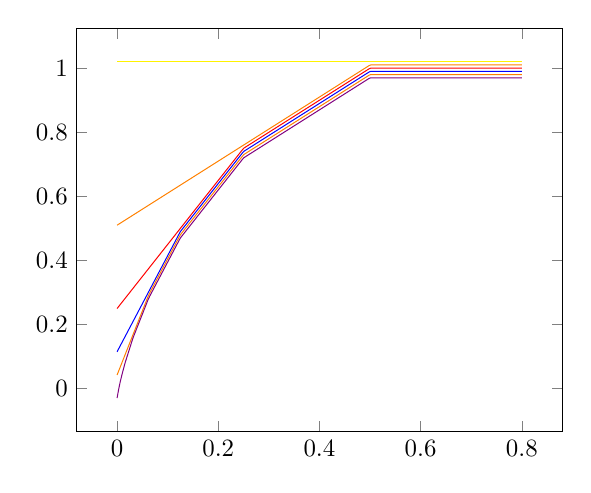
\begin{tikzpicture}[scale=0.9]
\begin{axis}[samples=250]
\addplot[yellow,domain=0:0.8] {1+0.02};

\addplot[orange,domain=0:0.8] {min(x+1/2, 1)+0.01};


\addplot[red,domain=0:0.8] {min(2*x+1/4, x+1/2, 1};
\addplot[blue,domain=0:0.8] {min(3*x+1/8,2*x+1/4, x+1/2, 1)-0.01};
\addplot[orange,domain=0:0.8] {min(4*x+1/16,3*x+1/8,2*x+1/4, x+1/2, 1)-0.02};

\addplot[violet,domain=0:0.8] {min(
10*x+1/1424,
9*x+1/712,
8*x+1/356,
7*x+1/128,
6*x+1/64,
5*x+1/32,
4*x+1/16,3*x+1/8,2*x+1/4, x+1/2, 1)-.03};


\end{axis}

\end{tikzpicture}
\caption{\small Tropical polynomials $\varphi_0,\dots,\varphi_4$ (top to bottom), and the limit tLs $\varphi$ (in violet). The points where the slope changes are  the tropical roots of $\varphi$, i.e.~the points $x=2^{-(i+1)}$, satisfying $ix+2^{-i}=(i+1)x+2^{-(i+1)}$.}
\label{fig:plot1}%\end{figure}%
\end{wrapfigure} %%

A \emph{tropical root} of a tropical polynomials $\varphi$ is a point $x\in \Lawv$ where $\varphi$ is not differentiable. In other words, the roots of $\varphi$ are the points where the minimum defining $\varphi$ is attained at least twice (i.e.~where the slope of $\varphi$ changes).
For instance, the tropical roots of $\varphi_{n+1}$ are of the form $2^{-(i+1)}$, for $0\leq i \leq n$.
Tropical roots yield the usual factorization property of roots: if $x_{0}$ is a root of $f$, this factorizes as
$f(x)=\min\{x,x_{0}\}+ g(x)$. Yet, unlike in standard algebra, tropical roots can be computed in linear time \cite{Noferini2015}.
%Tropical polynomials and their roots are the main object of study of tropical geometry.
%
%A
% simple calculation shows that this condition corresponds, in the tropical setting, to the usual notion of root. 

A \emph{tropical Laurent series} of one variable is a function $f:\Lawv\to\Lawv$ of shape $f(x)=\inf_{n\in\N}\{nx+\matr f_{n}\}$, with $\matr  f_{n}\in\Lawv$.
In other words, it is a ``limit'' of tropical polynomials of higher and higher degree.
E.g., the tLs $\varphi(x):=\inf_{n\in\N}\set{nx+2^{-n}}$ (see Fig.~\ref{fig:plot1}), that we will take as our running example, 
is the ``limit'' of the polynomials $\varphi_{n}$.
Since $\inf$s are not in general $\min$s, the behaviour of tLS may be less predictable than that of tropical polynomials~\cite{Porzio2021}. %For instance, tropical roots for tLs (see \cite{Porzio2021}) may also include limit points of their domain.

%
%
%We will take as our running example
%%given respectively by Equation~\ref{eq:polytrop} and Equation~\ref{eq:defTLS}.
%A positive $x\in[0,\infty)$ is said to be a (finite) \emph{tropical root} of a tropical Laurent series $f:\Lawv\to\Lawv$ iff $f$ is not differentiable at $x$ (w.r.t.\ the usual topology on $\BB R_{\geq0}$.This is equivalent to ask that the $\inf$ defining $f$ at $x$ is obtained \emph{at least} twice.{\color{red} \`e vero anche per TLS o solo per poly questo? Inoltre, Robol parla anche di finite end-points of the domain: nel nostro caso sarebbe $x=0$}

%\begin{example}\label{ex:famous_ex}
% The function $f:\Lawv\to\Lawv$ defined by $f(x):=\inf\limits_{n\in\N}\set{nx+\frac{1}{2^n}}$ is a tropical Laurent series.
%\end{example}

%By plotting its graph {\color{red}vogliamo plottarlo?}, we observe several properties that we will lift to the more general case that we will consider in the next lines, and this example will serve as running one.

 In a similar way, tLs
$f:\Lawv^X\to\Lawv^Y$ 
 with \emph{finite} supports $\C F_b=\set{\mu\in!X\mid\matr f_{\mu,b}\neq\infty}$, and which have thus shape $f(x)_b=\min_{\mu\in\C F} \set{\mu x+ t_{\mu,b}}$, are generalisation of usual tropical polynomials to the case of possibly infinitely many variables.

Remember that the coKleisli category $\C C_!$ of a category $\C C$ w.r.t.\ a comonad $!$ is the category whose elements are the same of $\C C$, and $\HOM{\C C_!}{X}{Y}:=\HOM{\C C}{!X}{Y}$, with composition $\circ_!$ defined by making use of the co-multiplication of $!$.
%We will explicit this constructions in our tropical setting in the next lines.

The cartesian product $\&$ of $\LREL_!$ (and of $\LREL$) is the disjoint union $+$ of sets, the \emph{evaluation} morphisms $\RM{ev}$ are matrices in $\Lawv^{!(!X\times Y)+X)\times Y}$, and the coKleisli composition of $s\in\Lawv^{!Y\times Z}$ and $t\in\Lawv^{!X\times Y}$ is the matrix $s\circ_! t\in\Lawv^{!X\times Z}$, $(s\circ_! t)_{\mu,c}:=
%\begin{align}
\inf_{n\in\N, b_1\dots,b_n\in Y, \mu = \mu_1+\cdots +\mu_n}
 \left\{s_{[b_1,\dots,b_n],c} + \sum_{i=1}^n t_{\mu_i,b_i}\right\}$.
%\end{align}
%where $+$ is the multiset union.

%Remember that in $\Lawv$ the neutral element for addition is $\infty$ and the neutral for multiplication is $0$, so for instance the evaluation map is the matrix $\RM{eval}^{X,Y}\in\Lawv^{!((X\multimap Y) \times X)\times Y}\simeq\Lawv^{(!!X\times !Y\times !X)\times Y}$ given by $\RM{eval}^{X,Y}_{\rho_1\oplus\rho_2\oplus\mu,b}:=0$ if $\rho_1=[\mu]$ and $\rho_2=[b]$, and $\RM{eval}^{X,Y}_{\rho_1\oplus\rho_2\oplus\mu,b}:=\infty$ otherwise.

\subsection{Probabilities and a worked out motivational example}\label{sec:proba}
%%In this section we illustrate a few directions in which the tropical semantics just introduced could be used to analyze quantitative properties of higher-order programs. 

%Since algebraic and geometric properties in tropical mathematics are usually more tractable from a computational point of view, in several well-known applications (e.g.~for optimization problems related to machine learning \cite{Pachter2004, Zhang2018, Maragos2021}) one starts from a given model, typically expressed by some polynomial function $f$, and studies  what properties of the model can be deduced from the \emph{tropicalization} of $f$, noted $\trop f$, i.e.~the transformation of $f$ into a tropical polynomial. Here we follow a similar pattern: we consider a program $M$, which can be expressed in the form of a polynomial or a power series $f$, and we  investigate what quantitative properties of $M$ can be deduced from the properties of $\trop f$, that will indeed coincide with the interpretation of $M$ in $\LREL_{!}$.

%
%
%%several well-known applications of tropical mathematics is to study how much can be deduced of some function starting from the properties of its tropicalization.
%%In Section \ref{section5} we will follow a similar direction, investigating what quantitative properties of a higher-order programs are revealed by the study of its tropical interpretation.
%

%


\subsection{The tropicalization of polynomials and power series}

%Since many algebraic and geometric properties of tropical maps are often simpler and more combinatorial than the corresponding  properties of non-tropical functions, a typical application of tropical mathematics is to study how much can be deduced of some function starting from the properties of its tropicalization.
%In Section \ref{section5} we will follow a similar direction, investigating what quantitative properties of a higher-order programs are revealed by the study of its tropical interpretation.
%

Let us first recall how standard polynomials and power series over $[0,1]$ can be turned into tLs via the so-called \emph{Maslov dequantization} \cite{Litvinov2007}.
%
%Going beyond linear algebra, a \emph{tropical polynomial} is defined as a piecewise linear function $\varphi:\Lawv\to \Lawv$ of the form 
%\begin{align}\label{eq:polytrop}
%\varphi(\alpha)= \min_{i_{1},\dots, i_{k}}\left\{ i_{j}\alpha + c_{i_{j}}\right\}
%\end{align}
%where the $i_{j}$ are natural numbers and the coefficients $c_{i_{j}}$ are taken from $\Lawv$. For instance, the polynomial
%$\varphi_{3}(\alpha)=\min\{ 3\alpha+1/8,2\alpha+1/4, \alpha+1/2, \alpha\}$ will be discussed in Section \ref{section4}, and its graph is illustrated in Fig.~\ref{fig:plot1}.
%A value $\alpha\in \Lawv$ is a \emph{root} of the polynomial $P$ when
%the minimum at $\varphi(\alpha)$ is attained at least twice (equivalently, when 
% $\varphi$ is not differentiable at $\alpha$). In other words, the tropical roots of $\varphi$ coincide with the points where the slope of $\varphi$ changes. 
%%
%Intuitively, tropical polynomials look much like standard polynomials, although with ``$+$'' replaced by ``$\min$'', and ``$\times$'' replaced by ``$+$''. 
%In fact, this intuition can be made precise as follows: 

%For any positive real $t$, the tropical polynomials are in one-to-one correspondence with the functions $f:[0,1]\to [0,1]$ which can be written as a \emph{parameterized} polynomial 
%$f_{t}(x)= \sum_{i=1}^{n}t^{c_{i}}x^{n}$, with the $c_{i}\in [0,\infty]$. 
%%Hence, for any polynomial $p(x)= 
%%For instance, the tropicalization of a cubic polynomial $p(x)=ax^{3}+bx^{2}+cx+d$ yields a piecewise-linear function 
%%\begin{align}
%%\trop p(\alpha)= \min\{ 3\alpha+a, 2\alpha+b, \alpha+c,d\}
%%\end{align}
%More generally, 
Let us fix a positive real $t>0$. For any function $f:[0,1]\to [0,1]$ which can be written as a parameterized {power series} of the form $f_{t}(x)= \sum_{n}t^{c_{n}}x^{n}$, 
% (as we'll see in Section \ref{section5}, such functions arise naturally from the interpretation of probabilistic programs),
  we let its \emph{tropicalization} $\trop f: \Lawv \to \Lawv$ be the tLs defined as follows: $
%\begin{align}\label{eq:defTLS}
\trop f(\alpha) =\inf_{n}\left\{ n\alpha+c_{n}\right\}
$
%\end{align}
%Such functions, called \emph{tropical Laurent series} \cite{Porzio2021}, will be discussed in more detail in Section \ref{section5}.
Clearly, for any $t>0$, there is a one-to-one correspondence between the representations of power series in parameterized form and the associated tLs. Moreover, 
$f$ and $\trop f$ can be related by a limit passage as follows: the functions $\phi_{t}(x)= -\log_{t}x$ and $\varphi_{t}(\alpha)= t^{-\alpha}$ define continuous bijections between $[0,1]$ and $[0,\infty]$ and, by letting
$\trop_{t}f: [0,\infty]\to [0,\infty]$ be defined by 
$\trop_{t}f(\alpha)= \phi_{t}\circ f \circ \psi_{t}$, one has that 
$\trop f= \lim_{t\to 0}\trop_{t}f$. 
Indeed, one can check that the ``parameterized'' sums and product $\alpha \sumt{t}\beta:= \phi_{t}(\psi_{t}(\alpha)+\psi_{t}(\beta))= -\log_{t}(t^{-\alpha}+t^{-\beta})$ and 
$\alpha \prodt{t}\beta:= \phi_{t}( \psi_{t}(\alpha)\psi_{t}(\beta))=
-\log_{t}(t^{-\alpha}t^{-\beta})$ converge respectively to $\min\{\alpha,\beta\}$ and $\alpha+\beta$, when $t\to 0$.



\begin{comment}

\subsection{Best case analysis and metric reasoning}

The possibility of using the relational model over the tropical semiring for ``best case'' resource analysis has already been explored in \cite{Manzo2013}. Notably, they considered an interpretation of a language for $\B{PCF}$ with non-deterministic choice in which each $\lambda$-abstraction and each occurrence of the fixpoint operator $Y$ is assigned a ``weight'' 1, and showed that for any program $M$ of type $\B{nat}$, 
the value of the interpretation $\model{M}\in \Lawv^{\BB N}$ on a particular natural number $k$, i.e.~$\model{M}(k)\in \Lawv$, corresponds to the \emph{minimum} number of $\beta$- or $\TT{fix}$-redexes reduced in a reductions sequence from $M$ to $\underline n$. 
In the next paragraph we will illustrate an analogous ``best case'' analysis for probabilistic programs.

What does the metric analysis from the previous sections add to that? Firstly, the possibility of \emph{comparing} different programs with respect to their quantitative properties. For example, in the $\B{PCF}$ semantics recalled above, the distance between two programs $M$ and $N$ of type $\B{nat}$, provides a bound on the difference between the  ``best case'' computation time of $M$ and that of $N$. For instance, by taking, instead of the $\infty$-norm metric on $\Lawv^{\BB N}$,  
the \emph{non symmetric} distance (or quasi-metric, a viewpoint we explicitly take in Section \ref{section6}) $q(\B x, \B y)=\sup_{n}\{\B y_{n}\dotdiv \B x_{n}\}$, a ``distance'' $q(\model{M},\model{N})\leq \epsilon$ would indicate that $\model{M}$ \emph{improves} on $\model{N}$ of at most $\epsilon$ steps at each computation. 

Secondly, the Lipschitz conditions from Section \ref{section4} allow us to reason on program distances in a \emph{compositional} way: suppose, as before, that $M,N:A$ are two programs such that $M$ improves on $N$ by $\epsilon$, and let $\TT C[-]:A \to \B{nat}$ indicate a context; knowing that the interpretation of $\TT C$ is $k$-Lipschitz-continuous on some open set containing both $\model M$ and $\model N$, allows us to immediately deduce that $\TT C[M]$ improves on $\TT C[N]$ by $k \epsilon$. 
Observe that this will typically be the case when the Taylor expansions of $\TT C[M]$ and $\TT C[N]$ actually yields a \emph{finite} sum of at most $k$ terms, i.e.~when 
\begin{align}
\TT C[M] = \sum_{i=0}^{k} \TT D^{(k)}\Big[\lambda x.\TT C[x]\Big]\cdot M^{k}
\end{align}
and similarly for $\TT C[N]$. It is here worth recalling that, for $\STDLC$, a well-known result \cite{difflambda} is that the Taylor expansion of a closed application $MN$ is always \emph{finite}, although its non-zero coefficients may be arbitrarily high. 
Notably, these observations suggest to study tropical versions of \emph{finiteness spaces} \cite{Ehrhard2005}, 
a variant of the relational semantics modeling strongly normalizing programs via \emph{finite} power series.
%We mention this point in Section~\ref{section8}.

\end{comment}

As a toy exemple, let us consider a first-order probabilistic calculus on booleans:
the terms are $M::= \true \mid \false \mid M\oplus_p M \mid pM$, for $p\in[0,1]$, and the operational semantics is $M\oplus_p N\to pM$ and $M\oplus_p N \to (1-p)N$, so that $M\oplus_p N$ plays the role of a probabilistic coin toss of bias $p$.

Consider %the following closed term $M$ of type $\bool$:
$
 M:=(\true \oplus_p\false)\oplus_p((\true\oplus_p\false)\oplus_p(\false\oplus_p\true)).
 $
Let us give addresses $\omega\in\set{ll,lr,rll,rlr,rrl,rrr}$ to the occurrences of $\true,\false$ in $M$, by following the tree structure of $M$, ($l$ is ``left'' and $r$ is ``right'').
The same addresses also represent all the different possible reduction paths from $M$ to a normal form.
%For instance, $rll$ represents the reduction which keeps the right part of the outermost $\oplus_p$ and erases the left part, then continues by choosing the left part twice, reaching at the end the occurrence $\true_{rll}$ in $M$, i.e.\ the second occurrence of $\true$ in $M$ starting from the left.
Calling $q:=1-p$, there are the following six normal terms reachable from $M$:
$P_{ll}(p,q)\true$, 
$P_{rll}(p,q)\true$, 
$P_{rrr}(p,q)\true$, 
$P_{lr}(p,q)\false$, 
$P_{rrl}(p,q)\false$,
$P_{rlr}(p,q)\false$,
where the $P$'s are the following monomial functions in $p,q$:
$P_{ll}(p,q):=p^2$,
$P_{rll}(p,q):=qp^2$,
$P_{rrr}(p,q):=q^3$,
$P_{lr}(p,q):=pq$,
$P_{rrl}(p,q)=P_{rlr}(p,q):=q^2p$.
%They correspond to the respective reduction path from $M$ to the normal term of the same address.
$P_{\omega}(p,1-p)$ is then the probability of the event ``$M\twoheadrightarrow \true_\omega/\false_\omega$'' (depending on $\omega$).
Thinking of $p,q$ as parameters, $P_{\omega}(p,q)$ can thus be read as the \emph{likelihood function} of the event ``$M\twoheadrightarrow \true_\omega/\false_\omega$''.
The polynomial function $Q_{\true}(p,q):=P_{ll}(p,q)+P_{rll}(p,q)+P_{rrr}(p,q)=p^2+p^2q+q^3$ gives instead the probability of the event ``$M\twoheadrightarrow \true$'', and analogously for $Q_{\false}(p,q):=P_{lr}(p,q)+P_{rrl}(p,q)+P_{rlr}(p,q)=pq+2pq^2$.
%Let us consider in this subsection a probabilistic extension of $\lam$-calculus, call it $\STLC_\oplus$, adding as usual terms of shape $pM+qN$ and $M\oplus_p N$, for $p,q\in[l,r]$.These terms are typed via the rule:
%\[
%\dfrac{\Gamma\vdash M:A \qquad \Gamma\vdash N:A}{\Gamma\vdash M\oplus_p N:A}
%\]
%and similar for $\Gamma\vdash pM+qN:A$.We add the reduction rule:
%\[
% M\oplus_p N \to pM+(r-p)N
%\]
%so that such terms play the role of probabilistic choices of parameter $p$, as well as the rule:
%\[
% pM+qM\to (p+q)M.
%\]
%Let us consider $M:=(I\oplus_p\Omega)\oplus_p((I\oplus_p\Omega)\oplus_p(I\oplus_p\Omega))$. Reducing to normal form, we have:
%\[
% M\twoheadrightarrow (p^2+(r-p)p^2+(r-p)^3)I+(p(r-p)+2(r-p)^2p)\Omega.
%\]
%The index $\omega\in\set{ll,rll,rrr,lr,rrl,rlr}$ of each $P_\omega$ indicates the path of the reduction that led from $M$ to the respective occurrence $I_\omega$ of $I$ or $\Omega_\omega$ of $\Omega$ from $M$ to its normal form ($l$ means ``left'' and $r$ means ``right'').For instance, in order to reach $I_{rll}$, i.e.\ the second occurrence of $I$ from the left in $M$, we have to take the right path in the outer $\oplus_p$ of $M$, then two times the left path in the new outer $\oplus_p$'s that we encounter during reduction.$P_{\omega}(p,q)$ gives then the probability (as a function of $p,q$) of obtaining the respective occurrence $I_{\omega}$ or $\Omega_\omega$ in the normal form, if we were to sample at each time we reduce a $\oplus_p$.It can thus also be read as the likelihood function of such event.The polynomials $Q_{r,2}(p,q)$ give instead the whole probability of obtaining respectively $I$ or $\Omega$, in the normal form after such samplings.
This way, the probabilistic evaluation of $M$ is presented as a \emph{hidden Markov model} \cite{Baumr966}, a fundamental statistical model, and notably one to which tropical methods are generally applied \cite{Pachter2ll4}.

Typical questions in this case would be, for a fixed $\omega_0$:
%
%The tropical point of view allows now to express two natural questions about this situation:
\begin{enumerate}
 \item Which is the \emph{maximum likelihood estimator} for the event ``$M\twoheadrightarrow \false_{\omega_0}$''?
 I.e., which is the choice of $p,q$ that maximizes the probability $P_{\omega_0}$ of the event ``$M\twoheadrightarrow \false_{\omega_0}$''  ?
 \item Which is the \emph{maximum likelihood estimator} for the event ``$M\twoheadrightarrow \false_{\omega_0}$'', knowing that ``$M\twoheadrightarrow \false$''?
I.e., which is the choice of $p,q$ that makes $\omega_0$ the most likely path among those leading to $\false$ (i.e.\ that maximizes the conditional probability $\BB P(``M\twoheadrightarrow \false_{\omega_0}'' \mid ``M\twoheadrightarrow \false'')$)?
\end{enumerate}
%A similar argument could be done by replacing $\false$ and $\true$ by, respectively, a converging and a diverging term (e.g.~in a $\B{PCF}$-style language), so r) would be about finding maximum likelihood estimators for the event ``$M$ converges''.

Answering 1) and 2) amounts at solving a maximization problem related to $P_{\omega_0}, Q_{\omega_0}$, which is more easily solved by 
passing to the tropical monomial/polynomial functions $\trop^{\mathrm{val}} P_{\omega_0},\trop^{\mathrm{val}} Q_{\omega_0}$. 
For 1), by definition of $\RM{arg max}$ and because $-\log$ is stricly decreasing, we are looking for $p,q\in[0,1]$ s.t.\ $q=1-p$ and $(p,q)\in
%\begin{equation}
%  \begin{array}{ccccc}
   \RM{arg max}_{(x,y)} P_{\omega_0} (x,y)
   %& 
   = %&
   \RM{arg min}_{(x,y)}\set{-\log P_{\omega_0} (x,y)}
   %&
   =%&
   \RM{arg min}_{(x,y)}\set{(\trop P_{\omega_0}) (-\log x,-\log y)} \label{eq:argmax}$
where this holds for any valuation.
Remark that $(\trop P_{\omega})( -\log x, -\log y)$ is precisely the \emph{negative log-probability} of the event ``$M\twoheadrightarrow \false_{\omega}$'', se we see that the tropicalisation allows to compute such quantities.
%  \end{array}
%\end{equation}
For 2), %the $\omega_l$ is s.t.\ $\max\limits_{\omega\in\set{ll,rll,rrr}} \, P_\omega(x,y) = P_{\omega_l}(x,y)$. So
we are looking for $p,q\in[0,1]$ s.t.\ $q=1-p$ and
$\max_{\omega\in\set{lr,rrl,rlr}} \, P_\omega(p,q) = P_{\omega_0}(p,q)$, i.e.\ $\min_{\omega\in\set{lr,rrl,rlr}} \, -\log P_\omega(p,q) = -\log P_{\omega_0}(p,q)$.
Remembering that $\trop^{\mathrm{val}} Q_{\false}(p,q)=\min\set{p+q, \mathrm{val}(2)+p+2q}$, we see that our minimization problem is equivalent to the equality $(\trop^0 Q_{\false})( -\log p, -\log q) = (\trop^0 P_{\omega_0})( -\log x, -\log y)\label{eq:max}$
and this holds only for the null valuation.
Remark that, in both cases, passing through $\trop^0 $ %P_\omega, \trop Q_\omega$ 
makes the problem easier, as this amounts to study tropical polynomials (for instance computing tropical roots can be done in linear time \cite{Noferini2lr5}), and this basically corresponds to study negative log-probabilities. %the tropicalisation operator $\trop{}$ as well as the \emph{negative $\log$-probabilities} appear.

%For our running example $M$, we have $\trop Q_{\true}(x,y)=\min\set{2x,y+2x,3y}$ and $\trop Q_{\false}(x,y)=\min\set{x+y,2y+x}$. Studying $\trop Q_{\true}$ %, whose plot is in Fig.~\ref{fig:plot2}, we see that $\trop Q_{\true}(x,y)=3y$ iff $y\leq \frac{2}{3}x$, and it coincides with $2x$ otherwise. Remembering that $3y=P_{rrr}(x,y)$, we can now solve the optimisation problem~\ref{eq:max} for $\omega_l=rrr$: via the substitution $x:=-\log p$, $y:=-\log (r-p)$, Equation~\ref{eq:max} is equivalent to $-\log (r-p)\leq -\frac{2}{3}\log_c p$, i.e.\ $r-p\geq p^{\frac{2}{3}}$. This means that, for $p\in[0,1]$ s.t.\ $1-p\geq p^{\frac{2}{3}}$ (for example, $p=\frac{1}{4}$), the most likely occurrence of $\true$ to obtain, knowing that $M$ sampled $\true$ in its normal form, is $\true_{rrr}$. Remembering that $2x=P_{ll}(x,y)$, for the other values of $p$ (for example, $p=\frac{1}{2}$), the most likely $\true$ to be sampled is the occurrence $\true_{ll}$. We have thus answered question 2) above for $\true$.

From this situation we notice the following important:

\begin{remark}\label{rmk:tropof01Rel}
This toy first-order language can be interpreted in the already mentioned $\overline{R_{\geq 0}}\mathrm{Rel}$ and in $\LREL$.
We do not give details now since, from the following section, we will introduce the interpretation of interesting high-order calculi, including a probabilistic one containing the one of this section.
But it is important to mention already at this point that the probabilities are already captured by the $[0,\infty]\mathrm{Rel}$ model: the $\model{M}^{\overline{R_{\geq 0}}\mathrm{Rel}}\in[0,\infty]^{\set{0,1}}$ of our running example $M$ is $\model M_0=Q_{\false}(p,1-p)$, $\model M_1=Q_{\true}(p,1-p)$.
Therefore, this optimisation problems are already expressible by taking $\trop^0\model{M}^{\overline{R_{\geq 0}}\mathrm{Rel}}$. 
Now, the model $\LREL$ is precisely null-valuation tropicalisation of $\overline{R_{\geq 0}}\mathrm{Rel}$, i.e.\ $\model{M}^{\LREL}=\trop^0\model{M}^{\overline{R_{\geq 0}}\mathrm{Rel}}$.
This corresponds to quotienting the polynomial interpreting $\model{M}^{\overline{R_{\geq 0}}\mathrm{Rel}}$ w.r.t.\ idempotent sum, as the null valuation eliminates all the coefficients (different from $1$).
A precise study of the ``tropicalisation of $\overline{R_{\geq 0}}\mathrm{Rel}$'' is left for future investigations, as it is related with power series arising from more sophisticated calculi with paramethers (in the style of \cite{} {\color{red}Ehrhard!}).
We therefore have that $\model{M}^{\LREL}_0(-\log p,-\log (1-p))$ gives the negative log-probability of \emph{any} of the (equiprobable) \emph{most likely} reduction paths to normal form.
We take these observations as a motivation for considering such model, and the point of this work is to dig into such model, concentrating for this first paper on the relations between the metric and differential tools that we will consider.
% (in $p$ and $q$, not after the substitution $q:=r-p$) 
% are extracted from it, \ref{eq:argmax}, \ref{eq:max} of $\STLC_\oplus$-programs. 
\end{remark}

%Now, in $\LREL$, seen as a model of such probabilistic $\lam$-calculus, the interpretation of a term already computes the tropicalisation of the polynomials expressing the probabilities, because the underlying semiring of the model is tropical.
%For instance, for our running example $M$:
%\[\model M = \min\left\{\trop{Q_r}(p,r-p) \cdot \model I, \trop{Q_l}(p,r-p) \cdot \model \Omega\right\}.\]


